\documentclass[11pt,a4paper]{article}

\usepackage{fontspec}
\setmainfont{PT Serif}
\setmonofont{PT Mono}[Scale=0.92]
\newfontfamily\headfont{PT Sans}
\usepackage[russian]{babel}
\usepackage[margin=2.2cm]{geometry}
\usepackage{booktabs}
\usepackage{graphicx}
\usepackage{xcolor}
\usepackage{array}
\usepackage{microtype}
\usepackage{enumitem}
\usepackage{hyperref}
\hypersetup{colorlinks=true, linkcolor=black, urlcolor={HTML}{1f4e79}, citecolor=black}

\definecolor{accent}{HTML}{1f4e79}
\definecolor{muted}{HTML}{555555}

\newcommand{\repsection}[1]{\vspace{1.1em}\noindent{\headfont\Large\bfseries\color{accent}#1}\vspace{0.35em}\par}
\newcommand{\repsub}[1]{\vspace{0.7em}\noindent{\headfont\large\bfseries\color{accent}#1}\vspace{0.2em}\par}

\setlength{\parskip}{0.55em}
\setlength{\parindent}{0pt}
\sloppy

\title{}
\date{}

\begin{document}

\begin{center}
{\headfont\LARGE\bfseries\color{accent} Премия за неликвидность на MOEX:\\[0.15em] кросс-секционная стратегия H-ILLIQ}\\[0.6em]
{\large Дмитрий Туминов}\\[0.15em]
{\small\color{muted} moex-backtest --- цикл 3 исследовательского трека CrossSectionalFactors \\ сентябрь 2026}
\end{center}

\vspace{0.3em}
\hrule
\vspace{0.9em}

\repsection{Резюме}

Стратегия покупает 9 наименее ликвидных бумаг из 47-именной вселенной MOEX и шортит 9 наиболее ликвидных, равными долями внутри каждой ноги, с месячным ребалансом. Ликвидность измеряется трейлинговым средним дневным оборотом (\texttt{VOLUME}~$\times$~\texttt{CLOSE}) за 252 торговых дня. Издержки --- 15~б.п. с оборота позиции, gross exposure 2.0.

На out-of-sample периоде 2022-01-31--2026-08-31 (56 месячных формаций) стратегия даёт годовой Sharpe~+1.087 при DSR~0.9797 (mechanism-scoped N=6), walk-forward efficiency 93.2\% и широком плато чувствительности по lookback (10--24 месяца дают 0.97--1.13). In-sample период 2018--2021 даёт Sharpe~+0.674 при p=0.076 --- сигнал на входе слабый, гейт пройден не с большим запасом.

Результат независимо переcчитан на втором движке (ziplime, тот же движок, что использует облачная инфраструктура Финама) на тех же данных: OOS Sharpe~+0.984 против наших +1.087, корреляция помесячных доходностей на 56 общих месяцах --- 0.929, средняя разница --- 1.19~п.п. в месяц. Разрыв по Sharpe (0.103) заранее, до запуска, был зафиксирован как порог 0.2 для поиска бага в реализации; фактический разрыв ниже порога и объясняется известными различиями конвенций, а не ошибкой.

Три ограничения делают +1.087 верхней границей, а не точечным прогнозом. Во-первых, смещение выживаемости не оценено количественно: вселенная отобрана как ликвидная в 2026 году и не содержит имён, делистингованных за 2018--2026 --- в архиве Мосбиржи через Finam Trade API найдено 267 архивных инструментов, из них порядка ста без преемника в текущей вселенной, и как минимум один документированный случай (URKA, июнь 2019) торговался в девять раз тоньше самой тонкой бумаги нынешней длинной ноги. Во-вторых, эффект режимно-зависим: короткая нога на 71.2\% состоит из 15 санкционных мегакапов, и исключение этих имён снижает OOS Sharpe до 0.827, а собственный IS-сигнал 32-именной версии (p=0.107) не прошёл бы гейт как новая гипотеза. В-третьих, 2025 год отрицателен на обоих независимых движках (наш −0.150, оракул −0.138 суммарной доходности) --- эдж сосредоточен в 2022 и 2026 годах, а не размазан равномерно.

\repsection{Экономическое обоснование}

Гипотеза H-ILLIQ: трейлинговый средний дневной оборот в рублях предсказывает доходность следующего месяца с обратным знаком --- наименее ликвидные имена систематически переигрывают наиболее ликвидные на риск-скорректированной основе, компенсируя держателю издержку входа и выхода. Это механизм компенсации за немедленность (Amihud \& Mendelson, 1986; Amihud, 2002), не поведенческая история о недо- или переоценке информации: чем труднее закрыть позицию без движения цены, тем выше требуемая доходность держания.

На MOEX это не абстрактная закономерность из учебника. По данным биржи, 70.7\% объёма торгов акциями в 2025 году пришлось на розничных инвесторов --- участников, которые торгуют небольшими объёмами, не предоставляют котировки на two-sided основе и не арбитражируют премию за ликвидность между именами так, как это делают профессиональные маркет-мейкеры. Институциональный арбитражный капитал, который в нормальных условиях должен был бы стирать эту премию, после 2022 года в значительной степени отрезан от рынка санкциями. Тот же аргумент о посттсанкционной сегментации капитала применяется здесь с не меньшей, а даже большей силой, чем в отклонённых гипотезах momentum и low-volatility (циклы 1--2 этого трека): сегментация напрямую снижает предложение капитала, готового ценить премию за неликвидность эффективно.

Это прямое следствие гипотезы, а не подгонка постфактум: направление (long неликвид, short ликвид) зафиксировано в преregistration до просмотра OOS-доходностей, а усиление эффекта именно после 2022 года --- предсказанное, а не обнаруженное свойство механизма. Раздел «Результаты» показывает, что OOS Sharpe (+1.087) превышает IS Sharpe (+0.674) --- инверсия, нетипичная для этого трека (momentum цикла 1 давал обратное: IS~+1.624~$\to$~OOS~+0.562), и она согласуется с этим прогнозом, но не доказывает его: один цикл не может отличить «механизм структурно усилился после 2022» от «OOS оказался благоприятной выборкой».

\repsection{Методология и pre-registration}

Гипотеза, вселенная, издержки, сетка параметров и критерии провала зафиксированы в \texttt{PREREGISTRATION\_cycle3\_illiquidity.md} 10.09.2026, до расчёта сигнала по доходностям --- это новый экономический механизм для проекта, зарегистрированный в \texttt{trial\_ledger.MECHANISM\_BY\_HYPOTHESIS} заранее, чтобы «momentum, пересобранный иначе» не мог тихо обнулить счётчик трейлов.

Единственный свободный параметр --- lookback трейлингового среднего оборота. Глубина ноги (\texttt{n\_per\_leg}=9, floor(47/5)) и период удержания (1 месяц) зафиксированы априори по той же причине, что и в циклах 1--2: перебор параметра, не являющегося самой гипотезой, провоцирует спайк, а не плато. Бюджет трейлов --- максимум 3 конфигурации (Phase~A1 с lookback=12, затем сетка \{3, 6, 12\} только если Phase~A1 проходит); если Phase~A1 не проходит, сетка не запускается и цена цикла для счётчика N равна ровно 1.

\begin{center}
\small
\begin{tabular}{ll}
\toprule
Параметр & Значение \\
\midrule
IS-период & 2018-01-01 -- 2021-12-31 \\
OOS-период & 2022-01-01 -- 2026-09-09 \\
Вселенная & 47 тикеров MOEX \\
Глубина ноги & 9 имён long, 9 short \\
Издержки & 15 б.п. одностороннего оборота \\
Gross exposure & 2.0 (каждая нога 100\% капитала) \\
Ребаланс & ежемесячный \\
\bottomrule
\end{tabular}
\end{center}

Финальный вердикт требует одновременного выполнения всех шести критериев гейта --- частичного зачёта нет: (1) значимость на IS по стационарному бутстрапу, p<0.10; (2) walk-forward, среднее OOS Sharpe > 0; (3) плато чувствительности по locked-параметру; (4) блочный Monte Carlo bootstrap, percentile~$\le$~95; (5) Deflated Sharpe Ratio при mechanism-scoped N > 0.95; (6) Probability of Backtest Overfitting < 0.5. Разделение IS/OOS физически закрыто локом конфигурации (\texttt{validation.lock.require\_locked\_config}) --- OOS-доходность не вычисляется ни одной строкой кода этого цикла до записи выигравшей конфигурации в \texttt{experiments/cycle3\_illiquidity.lock.json}, а не по договорённости «не подглядывать».

Счётчик трейлов для DSR --- mechanism-scoped, а не общепроектный: он считает только испытания того же экономического механизма, что и оцениваемый кандидат (\texttt{N\_CONVENTION.md}, принято 10.09.2026 после того, как общепроектный счётчик показал, что реальный эффект с историческим Sharpe~+0.562 не мог пройти гейт ни при каком объёме данных --- DSR дефлирует по числу перебранных гипотез, а не по количеству собранных наблюдений, и эта планка инвариантна к T). Для нового механизма счётчик стартует с нуля и наследует только собственные трейлы цикла. После первого прохода гейта (3 трейла, DSR~0.9833 при N=3) в цикл были добавлены три дополнительных, честно учтённых трейла для проверки двух конкретных возражений (ниже) --- итоговый mechanism-scoped~N=6, DSR пересчитан на тех же locked OOS-доходностях и составил \textbf{0.9797}. Общепроектный счётчик (context only, никогда не подставляется в формулу) вырос за это время с 10 до 16 --- приведён рядом как отдельное предупреждение Harvey/Liu/Zhu (RFS, 2016): исследователь, перебравший много разных аномалий за карьеру, должен быть скептичнее в целом, даже если ни один отдельный расчёт DSR этой истории не видит.

Леджер (\texttt{experiments/grid\_search\_log.jsonl}) append-only: каждая запись помечена \texttt{counts\_toward\_n}, диагностические прогоны (cost-sensitivity, dense sensitivity curve, ablation с 45 именами) идут с \texttt{counts\_toward\_n=false} и не входят в N ни для одной гипотезы --- это стресс-тест уже выбранного кандидата, а не новый отбор.

\repsection{Результаты}

\repsub{Гейт}

\begin{center}
\small
\begin{tabular}{lr}
\toprule
Критерий & Результат \\
\midrule
IS Sharpe (2018--2021) & +0.674, p=0.076 \\
OOS Sharpe (2022--2026, 56 мес.) & \textbf{+1.087} \\
Walk-forward efficiency & 93.2\% (mean OOS +0.895, 7 окон) \\
Sensitivity & плато (lookback 10--24: 0.97--1.13) \\
Monte Carlo percentile & 50.4 \\
DSR (mechanism-scoped N=6) & \textbf{0.9797} \\
PBO (3 трейла, 16 блоков) & 0.300 \\
OOS turnover & 6.1\% позиций/мес. \\
\bottomrule
\end{tabular}
\end{center}

Ни одна из этих цифр не проходит гейт с комфортным запасом равномерно. DSR имеет реальный запас над порогом 0.95 (E[max~SR$\mid$H0]=+0.199 против наблюдаемых +1.087 --- более чем шестикратный разрыв), а Monte Carlo percentile 50.4 --- это фактически середина нулевого распределения, самая нейтральная цифра, которую этот трек когда-либо фиксировал. Но Phase~A1 p=0.076 близок к отсечке 0.10, а PBO~0.300 хоть и укладывается в требование <0.5, находится вне «комфортной зоны» <0.2, которой проект неформально пользовался как ориентиром (для сравнения, momentum цикла 1: PBO=0.032). Низкий \texttt{trial\_sharpe\_variance} (0.023--0.037 на разных пересчётах, против 0.560 у momentum) --- то, что реально удерживает DSR высоким, а не mechanism-scoped N сам по себе: узкая сетка похожих трейлов по построению формулы дешевле проходит гейт, чем широкая, и это честный стимул держать сетку узкой по содержательной причине, а не инструмент для игры с DSR.

Оборот всего 6.1\% позиций в месяц --- на порядок ниже, чем у momentum (23.2\%): состав ног --- медленно меняющееся структурное свойство, а не то, что пересобирается заново каждый месяц. Это делает результат устойчивым к издержкам (при 100~б.п. вместо 15 Sharpe снижается лишь до +1.059), но одновременно означает, что линейная модель издержек «оборот $\times$ ставка» может недооценивать реальную стоимость первоначального набора позиции в тонких именах --- разовая просадка через стакан, которую помесячный оборот не отражает.

\repsub{Состав ног}

\begin{center}
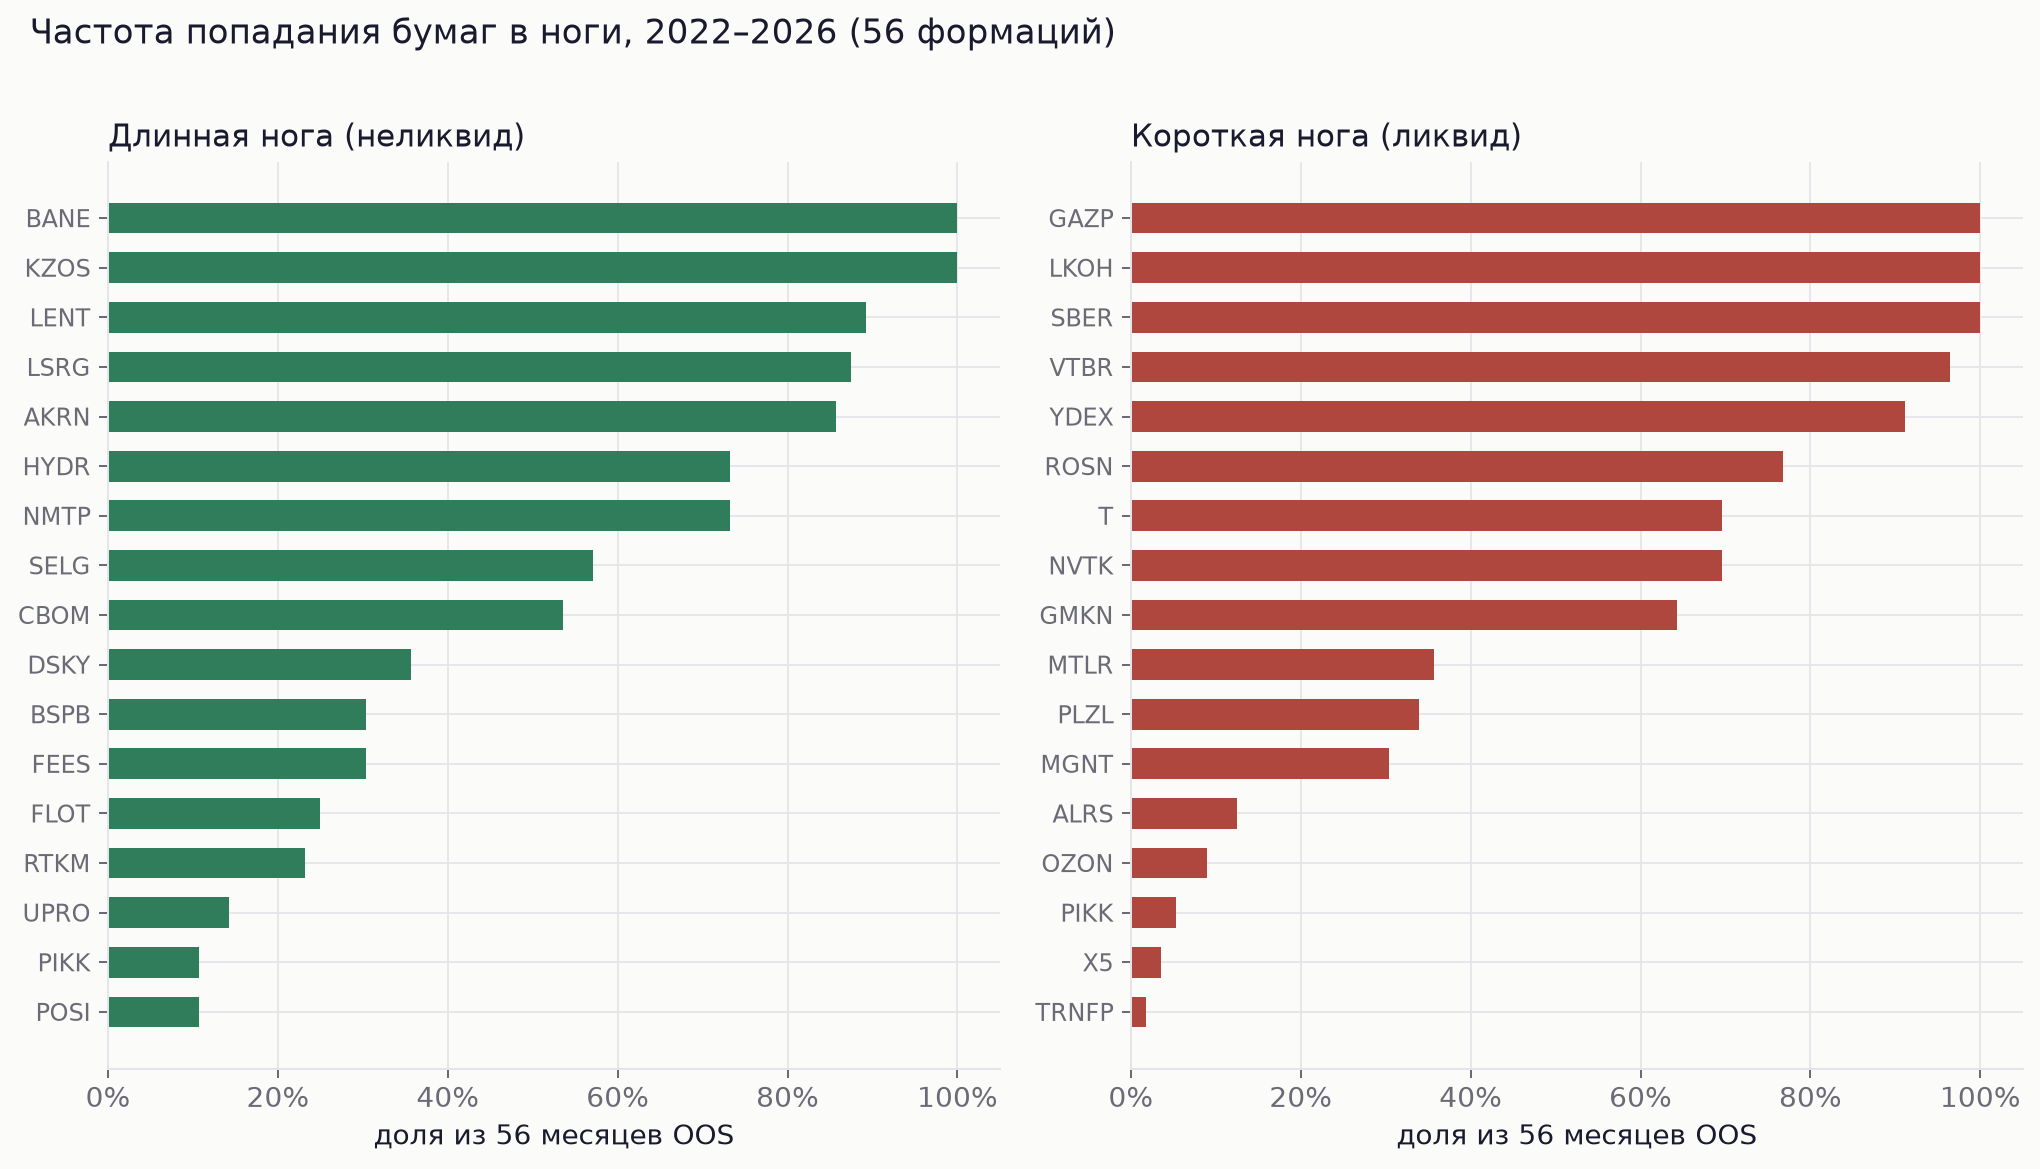
\includegraphics[width=\linewidth]{assets/leg_composition.png}
\end{center}

Состав ног намного ближе к почти статичной корзине, чем к жёсткой пересортировке каждый месяц. В длинной ноге BANE и KZOS присутствуют все 56 из 56 месяцев OOS, LENT --- 89\%, LSRG --- 88\%, AKRN --- 86\%. В короткой ноге GAZP, LKOH и SBER --- 100\% месяцев, VTBR --- 96\%. Реально задействовано 33 бумаги из 47 --- 14 имён (AFLT, ASTR, CHMF, IRAO, MAGN, MOEX, MTSS, NLMK, PHOR, RUAL, SIBN, SNGS, TATN, VKCO) не попали ни в одну ногу ни разу за весь период.

Это не превращает результат в историю про две-три удачные бумаги. Исключение двух стопроцентно постоянных имён (KZOS, BANE) из 45-именной версии вселенной почти не двигает OOS Sharpe (+1.026 против +1.087) --- и это несмотря на то, что сам KZOS за период OOS был убыточным (годовая средняя доходность −8.5\%), как и HYDR (−10.8\%, 73\% месяцев в ноге). Положительный Sharpe длинной ноги выживает вопреки убыточности двух самых постоянных её участников, что плохо согласуется с гипотезой «это просто пара удачных ставок». Разложение по ногам подтверждает то же самое отдельно: длинная нога сама по себе даёт OOS Sharpe +0.373 (средняя годовая доходность +10.7\%), короткая --- Sharpe −0.243 (−7.3\% годовых), при равновзвешенной доходности всей вселенной за то же окно около −1.3\% годовых. Обе ноги работают в предзарегистрированном направлении, ни одна не тащит результат в одиночку.

\repsection{Независимая верификация}

Реализация облачной инфраструктуры Финама построена на движке ziplime; тот же файл стратегии, тот же движок, версия 1.19.16 (последний релиз на PyPI на момент проверки, 18.06.2026, сверено по восьми кадрам собственного трейсбека движка) был поднят локально на тех же данных, с теми же параметрами, явно выставленными в коде: капитал 10~млн~₽, \texttt{max\_leverage=2.0}, исполнение по цене закрытия следующего бара, комиссия PerDollar(0.0015), без проскальзывания. Единственное отличие от продовой обвязки платформы --- импорт \texttt{MarketOrder}: облако подставляет имя в неймспейс алгоритма само, при локальном запуске файл импортируется как обычный модуль.

\begin{center}
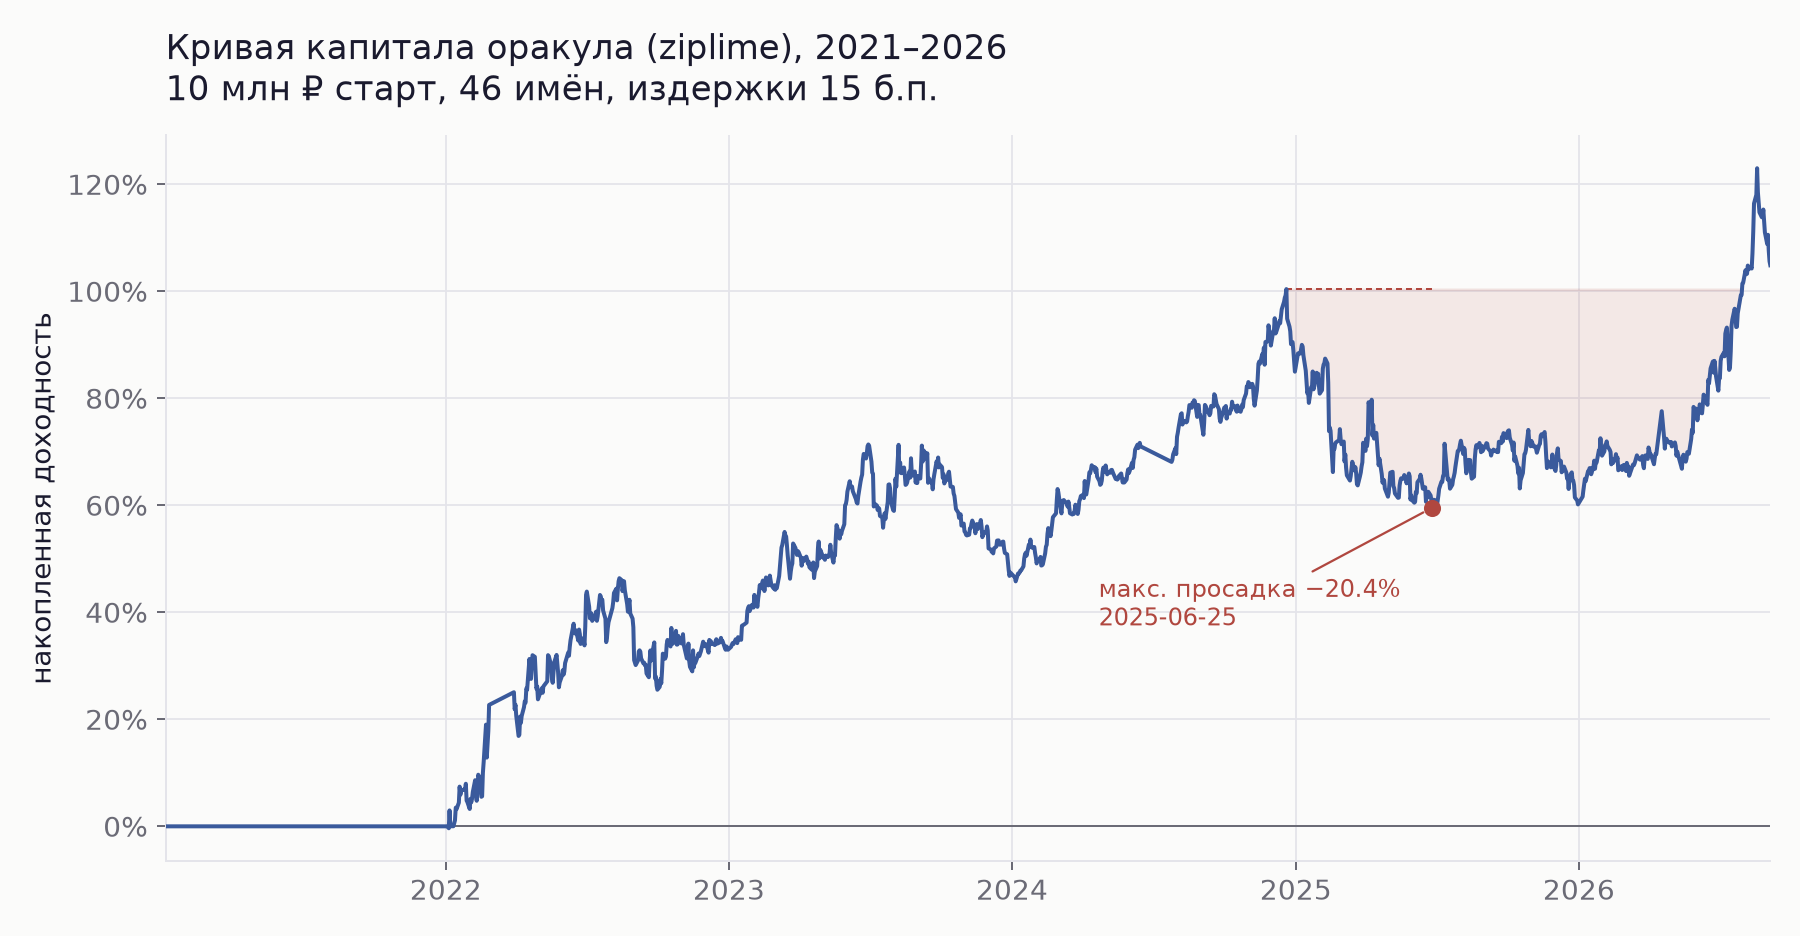
\includegraphics[width=\linewidth]{assets/oracle_equity_curve.png}
\end{center}

На периоде 2021-01-04--2026-09-04 (2021 год --- разогрев индикатора без позиций, реальная торговля с 2022 года) оракул превращает 10~млн~₽ в 20.49~млн: итог +104.9\% за 4.67 года, или +16.6\% годовых. Помесячный Sharpe +0.984 (дневной, аннуализированный через $\sqrt{252}$ --- +0.882), волатильность 16.3\%, максимальная просадка −20.4\% с пиком 25.06.2025 --- продолжительный, почти годовой период боковика после сильного роста 2024 года, а не резкий обвал.

\begin{center}
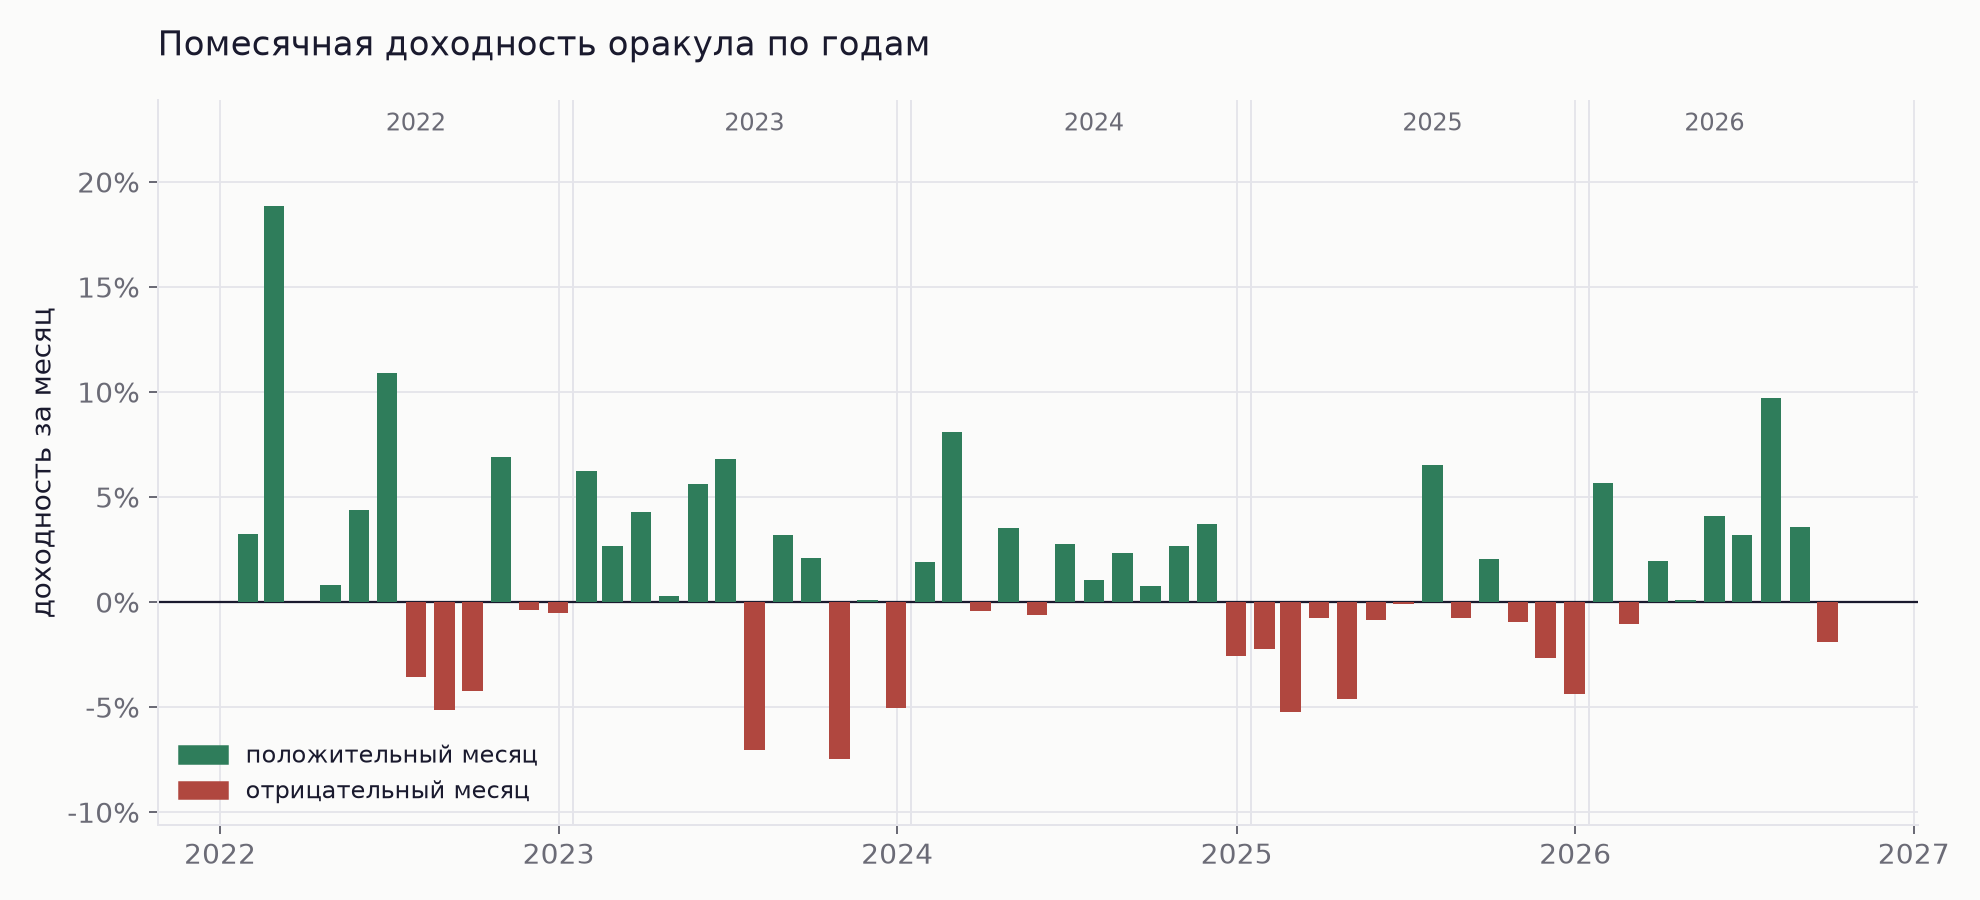
\includegraphics[width=\linewidth]{assets/oracle_monthly_returns.png}
\end{center}

Помесячная картина показывает то же, что и сводка по годам: лучшие месяцы --- февраль 2022 (+18.8\%) и июнь 2022 (+10.9\%), формирование портфеля происходит по первому бару месяца, то есть до обвала конца февраля, и шорт мегакапов отрабатывает сам по себе, без использования постобвальной информации. Это разошлось с предварительным прогнозом: до прогона ожидалось, что исполнение следующим баром сделает февраль 2022 у оракула заметно слабее нашего результата (сигнал 25.02 не мог быть исполнен раньше 24.03) --- на деле оракул дал за февраль больше, а не меньше (+18.84\% против наших +16.49\%). Зафиксировано как несбывшееся предсказание, а не подогнано под факт постфактум.

Прямое сопоставление на 56 общих месяцах (формация месяца~M у нашего движка размечена как календарный месяц~M+1 у оракула, потому что оракул размечает доходность календарным месяцем удержания, а не датой формации):

\begin{center}
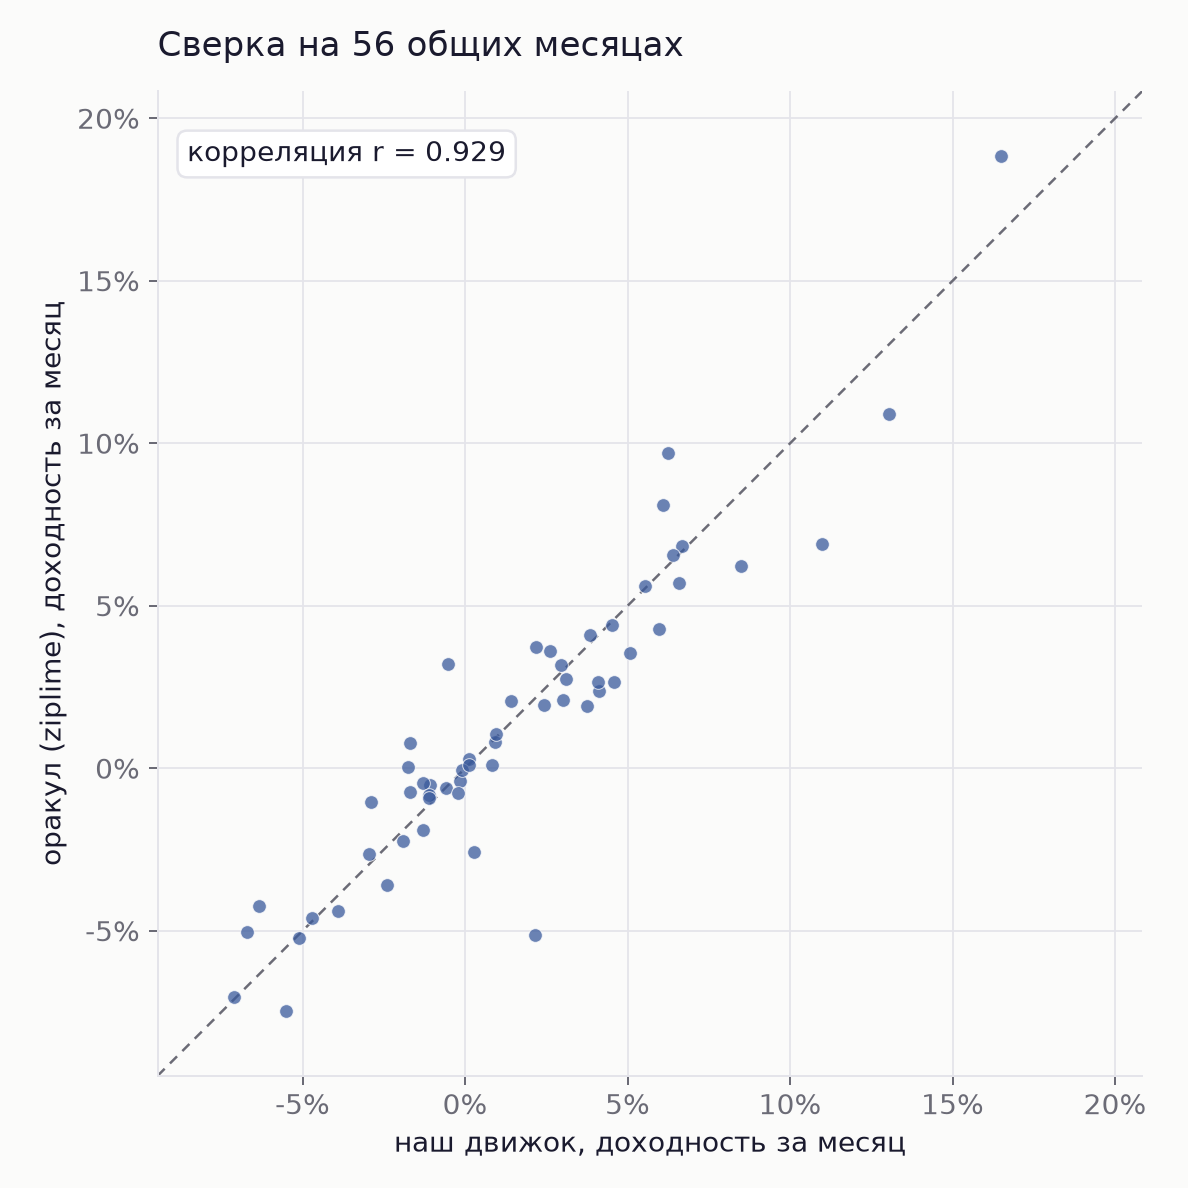
\includegraphics[width=\linewidth]{assets/engine_vs_oracle_scatter.png}
\end{center}

\begin{center}
\small
\begin{tabular}{lrr}
\toprule
 & наш движок (47 имён) & оракул ziplime (46 имён) \\
\midrule
Sharpe (56 мес.) & +1.087 & +0.984 \\
Сумма доходностей & +0.834 & +0.748 \\
\bottomrule
\end{tabular}
\end{center}

Корреляция помесячных доходностей --- \textbf{0.929}, средняя абсолютная разница --- 1.19~п.п. в месяц. Разрыв по Sharpe (0.103) был заранее, до запуска, зафиксирован как порог 0.2 --- повод искать баг в реализации, если превышен. Фактический разрыв ниже порога и объясняется известными различиями конвенций: издержки с каждого оборота против однократных при входе, исполнение на следующем баре, ребаланс по первому бару месяца против нашей разметки по дате формации, 46 имён у оракула против 47 (DSKY исключён --- см. ниже). По годам расхождение системное, не случайное: 2022 --- +0.364 у нас против +0.281 у оракула, 2023 --- +0.189/+0.118, 2024 --- +0.261/+0.233, 2025 --- $-0.150/-0.138$, 2026 (9 месяцев) --- +0.171/+0.255. Отрицательный 2025 год воспроизвёлся независимо на обоих движках --- это уже не особенность конкретной реализации, а свойство самого периода.

Независимая верификация обнаружила и настоящую ошибку в производственном коде сигнала, не в оракуле: \texttt{illiquidity\_signal} позволял устаревшей trailing-оценке DSKY удерживать бумагу в длинной ноге ещё около шести месяцев после того, как реальные данные по ней закончились (14.10.2024) --- механизм не артефакт reindex/ffill, а легитимное поведение \texttt{rolling(window=252, min\_periods=126)}, который всё ещё находит достаточно исторических наблюдений внутри окна. Явная маска по актуальности \texttt{close\_panel} сократила месяцы DSKY в ноге с 20 до 14 и дала OOS Sharpe +1.104 вместо +1.087 --- то есть баг не завышал прошедший гейт результат, если что и занижал его. Исправление зафиксировано как находка в \texttt{factors.py}, но не применено к уже прошедшему ревью коду без отдельного решения об этом.

Помимо независимой верификации, оракул на этом же прогоне вскрыл пять ошибок движка ziplime, не относящихся к самой стратегии (симуляция молча обрывается на дате делистинга участника вселенной без ошибки и без NaN в метриках; падение при отсутствии цены у открытой позиции в момент формирования собственного текста ошибки; падение при \texttt{benchmark\_asset\_symbol=None}; календарь XMOS не знает об остановке торгов MOEX в конце февраля -- марте 2022; файл алгоритма импортируется без инъекции неймспейса) --- подробности в \texttt{ORACLE\_RESULTS.md} независимого репозитория \texttt{finam-championship}.

\repsection{Ограничения и условия разворота}

\repsub{Смещение выживаемости --- признано, не измерено}

47-именная вселенная отобрана как «ликвидная» по состоянию на сентябрь 2026 года и ретроактивно применена ко всему окну 2018--2026. Любая компания, обанкротившаяся или делистингованная в этом окне и не входящая сегодня в топ-47 по ликвидности, невидима для этого исследования по построению. Через Finam Trade API (\texttt{AllAssets(only\_disabled=true)}) найдено 10\,115 архивных инструментов по всем биржам, из них 267 с MIC MISX и типом EQUITIES; после исключения 131 инструмента-зеркала иностранных компаний (\texttt{-RM}) и 36 депозитарных расписок компаний, уже присутствующих в текущей вселенной под основным тикером (принудительный делистинг ГДР с Лондонской биржи в 2022 году сменил форму листинга, но не компанию), остаётся \textbf{100 архивных имён без идентифицируемого преемника} --- реальный кандидатный пул, не гипотетический.

DSKY напрямую присутствует в этом списке с флагом \texttt{is\_archived: true} --- независимое живое подтверждение того, что уже видно на кэшированных данных: бумага провела 36\% своей OOS-жизни (20 из 56 месяцев) в длинной ноге до делистинга 14.10.2024. Более показательный пример --- URKA (Уралкалий): точечная проверка через API подтвердила торги в июне 2019 года, внутри собственного IS-периода этого цикла, с медианным дневным оборотом \textbf{2.35~млн~₽} --- почти в девять раз тоньше самой тонкой бумаги текущей вселенной (KZOS, 20.5~млн~₽/день по OOS-периоду). Компания реально существовала, реально торговалась на уровне ликвидности значительно ниже нижнего квинтиля текущего бэктеста и невидима для этого исследования только потому, что была делистингована.

Направление смещения однозначно: если компании, close to банкротства, становятся неликвидными до того, как обанкротиться (что экономически правдоподобно и согласуется с единственным разобранным примером), а бэктест способен наблюдать только те неликвидные имена, которые дожили до включения в вселенную 2026 года, то измеренная доходность длинной ноги --- оценка, обусловленная выживанием, смещённая в сторону завышения истинной премии за неликвидность. Величина смещения не оценена и не оценивается здесь: это требует точечной во времени исторической вселенной MOEX, реконструкция которой --- отдельный проект по данным (вероятно, платный источник или ручная архивная работа), сознательно не предпринятый в рамках этого цикла. \textbf{Следствие: +1.087 --- верхняя граница достижимой премии, а не точечный прогноз.}

\repsub{Режимная зависимость, не структурная премия}

Короткая нога на 71.2\% состоит из одних и тех же 15 санкционных мегакапов и системообразующих банков (GAZP, LKOH, ROSN, NVTK, TATN, SNGS, SIBN, GMKN, NLMK, CHMF, MAGN, RUAL, PLZL, SBER, VTBR) --- GAZP, SBER и LKOH в шорте все 56 из 56 месяцев OOS. Это не новость постфактум-2022: тот же состав на IS-периоде (2018--2021, до всех санкций) даёт даже более высокую долю --- 80.7\%. GAZP, SBER и LKOH были самыми ликвидными именами MOEX и до санкций --- «шортить самый ликвидный квинтиль» и «шортить системообразующие мегакапы» на этом конкретном рынке механически почти совпадают в обоих периодах, что ослабляет сильную форму возражения: конструкция не начала захватывать санкционные имена именно после 2022 года, она делала это всегда.

Изменилось поведение доходностей примерно той же корзины: на IS сигнал был слабым (Sharpe +0.674, p=0.076, едва внутри гейта Phase~A1), на OOS --- намного сильнее (+1.087) при почти неизменном составе ноги. Это ровно тот паттерн, который дала бы смена режима в относительной доходности мегакапов, а не изменение самой конструкции, и согласуется с (хотя и не доказывает) предзарегистрированный аргумент о посттсанкционной сегментации капитала.

Прямая проверка (пост-хок, после того как 47-именной OOS-результат уже был известен, что честно оговорено): исключение всех 15 санкционных мегакапов из вселенной целиком (32 имени, \texttt{n\_per\_leg}=floor(32/5)=6) даёт OOS Sharpe \textbf{+0.827} против локированных +1.087 --- снижение примерно на четверть. Собственный IS-сигнал этой 32-именной версии (p=0.107) как самостоятельная гипотеза не прошёл бы гейт Phase~A1. Вывод: эффект реален и переживает эту исключающую проверку, но не является чистой структурной премией --- он частично (примерно на четверть измеренного эджа) зависит от режима. \textbf{Условие разворота}: устойчивое возвращение иностранного арбитражного капитала на MOEX или существенное снятие санкций именно с этих 15 имён убрало бы эту четверть эджа; данных о том, что оставшиеся ~0.83 Sharpe сами по себе иммунны к более широкой смене режима, здесь нет --- проверена устойчивость только к этой конкретной абляции.

\repsub{2025 год отрицателен на обоих движках}

Суммарная доходность 2025 года --- $-0.150$ у нашего движка и $-0.138$ у оракула, независимо друг от друга. Эдж сосредоточен в 2022 и 2026 годах, а не распределён равномерно по всему окну. Пятилетнее окно с одним явно отрицательным годом на двух независимых реализациях --- часть картины, которую агрегированный Sharpe за весь период не показывает сам по себе.

\repsub{Эффективная широта ниже заявленной}

Пять имён (BANE, KZOS, LENT, LSRG, AKRN) держатся в длинной ноге в 86--100\% месяцев OOS --- это устойчивая ставка на горстку бумаг, а не перебор всей вселенной заново каждый месяц. Реально задействовано 33 бумаги из 47; остальные 14 не участвовали ни разу. Формальный n\_per\_leg=9 не отражает, насколько мала фактическая широта позиций.

\repsub{Издержки посчитаны не полностью}

15~б.п. с оборота позиции учтены, но не учтены: ставка займа по коротким позициям, проскальзывание при входе в тонкие имена и влияние собственных ордеров на цену. Для стратегии, вся экономическая логика которой строится на том, что тонкие имена дорого торговать, линейная модель издержек по обороту специфически недооценивает именно ту часть стоимости, ради компенсации которой стратегия существует. Реальный шорт по девяти именам также требует доступности бумаг для займа, а биржа сохраняет дискреционное право временно запрещать короткие продажи по отдельным бумагам --- задокументированный случай ЕвроТранса в июле 2026 года.

\repsub{Известная ошибка оракула}

Оракул считался без DSKY (46 имён вместо 47) из-за бага движка ziplime: симуляция с делистингованным участником вселенной в составе молча обрывается на дате его последней сессии, без ошибки и без NaN в итоговых метриках --- обнаружено и подтверждено минимальным повтором (без DSKY прогон идёт полные 1385 баров до 04.09.2026, с DSKY --- обрывается на 912 барах, день в день с последней сессией DSKY).

\repsection{Воспроизводимость}

Всё --- в каталоге \texttt{strategies/CrossSectionalFactors/}. Гипотеза, вселенная, издержки и критерии провала, зафиксированные до расчёта сигнала, --- в файле \texttt{PREREGISTRATION\_cycle3\_illiquidity.md}. Полный отчёт цикла, включая все диагностики и обе раунды разбора возражений, --- в \texttt{reports/cycle3\_illiquidity.md}. Конвенция подсчёта трейлов для DSR --- в \texttt{N\_CONVENTION.md}. Леджер трейлов (append-only, JSON Lines, каждая запись с меткой \texttt{counts\_toward\_n}) --- в \texttt{experiments/grid\_search\_log.jsonl}; лок выигравшей конфигурации, физически закрывающий доступ к OOS до фиксации параметра, --- в \texttt{experiments/cycle3\_illiquidity.lock.json}.

\begin{center}
\small
\begin{verbatim}
uv run python strategies/CrossSectionalFactors/run_cycle3_illiquidity.py
uv run python strategies/CrossSectionalFactors/trial_ledger.py   # текущие счётчики N
\end{verbatim}
\end{center}

Независимый оракул --- отдельный репозиторий \texttt{finam-championship}, движок ziplime~1.19.16, тот же файл стратегии (\texttt{algorithms/moex\_illiquidity.py}), те же данные через \texttt{moex\_bundle.py} (parquet-кэш \texttt{moex-backtest}, 47 тикеров, 2018-01--2026-09, 101\,119 строк). Полная методология сборки и все найденные расхождения --- в \texttt{ORACLE\_RESULTS.md} этого репозитория.

\begin{center}
\small
\begin{verbatim}
uv run python run_moex_oracle.py
\end{verbatim}
\end{center}

Графики этого отчёта построены по уже посчитанным данным (\texttt{oracle\_monthly\_returns.csv}, \texttt{oracle\_perf.pkl}, доходности нашего движка --- прямым вызовом \texttt{\_illiq\_returns} с уже локированным lookback=12 на уже размеченных OOS-датах) --- без повторного запуска гейта, без нового трейла, без изменения N.

\vspace{1.5em}
{\small\color{muted}\hrule\vspace{0.5em} Данные: MOEX ISS + Finam Trade API, кэш parquet, 47 тикеров, 2018-01-03--2026-09-09. Издержки: 15 б.п. одностороннего оборота, без учёта ставки займа и проскальзывания. Результат прошлого периода не является обязательством будущей доходности.}

\end{document}
